\section{Approach to optimization using NeuronUnit}
Model optimization follows the following basic approach:
\begin{enumerate}
	\item Identify a model class whose parameters are to be optimized, e.g. the Izhikevich model.
	\item Identify a neuron whose experimental data will be used to guide optimization.
	\item Identify a suite of tests that can use that experimental data to guide the optimizer.
	\item Execute optimization of that model class against that suite of tests to return an optimized model.
\end{enumerate}
Within these steps are also a number of smaller decisions, including where the experimental data will be obtained and what kind of simulator will be used to run the model.

Using NeuronUnit, the steps above take the follow pseudo-code form:

\begin{lstlisting}[language=python]
# Import code from NeuronUnit
from sciunit import TestSuite
from neuronunit.models import MyModelClass
from neuronunit.tests import MyTestClass1, MyTestClass2, MyTestClass3
from neuronunit.data import get_data_from_database_x

# Get data about my neuron
neuron_type = "Layer 5 pyramidal Neuron"
neural_data = get_data_from_database_x(neuron_type)
test1 = MyTestClass1(observation=neural_data)
test_suite = TestSuite([test1, test2, test3])
results = test_suite.optimize(model)
\end{lstlisting}

There are two different paradigms for evaluating models in neuronunit, under paradigm 1 the model is a supported by NeuronUnit, therefore dynamic simulation of the model are present on the host computer and cheap to re-run.

Under paradigm 2 the neuronunit model only consists of model inputs and outputs that are streamed as needed from a different environment this is because the true model is either very complex, and it would not improve clarity to re-implement the model again, or the true model is on a remote machine, and its outputs are accessed via an API. Another way of saying this is that if a "model" is simply a digitized set of waveform, converting it to a model, is as simple as labeling things such that neuronunit and the scientist are both consistent about what is a model and what isn't. The optimization procedures I describe in this work involve both paradigms, optimizing within the second paradigm required dedicated code, that are not supported within the other previously described frameworks.

\section{Model Class Implementations}
Because optimization may involve an extremely large number of independent simulations of the same class of model, each varying only in model parameter values, it is critical that both the overhead for model instantiation and the duration of simulation itself, be as low as possible. We built faster python implementations of two neuronal models (Izhikevich model and adaptive Exponential model). One of the implementations was based on MATLAB forward euler implementation of the Izhi model, another implementation of the Adaptive Exponential model came from vectorized python code, which was relatively slow.

I was able to use a tool \cite{numba} enables In Time compilation(JIT), to make both of these models perform faster than standard neuron simulator versions in brian2 and NEURON.
 %Without over stating things, 
 When regarding this thesis effort and its contribution to knowledge, some of the value to the neuroscience modelling community comes from the implementation of two fast python neural model simulations. Because these simulations are written in python, the code that implementations them is easy to understand share and execute, because the models are fast to dispatch they maybe useful in both network contexts, and optimization contexts where performance is critical. 
 
%A component of this work the Izhikevich model, I plan to push to the Open Source Brain %\href{https://github.com/russelljjarvis/IzhikevichModel.git}


\subsubsection{Why Existing Approaches Were Not workable}
In this research effort significant time was spent shoe-horning pre-existing tools into an optimization frame work, with limited success. These tools included:  PyNN, brain2, \emph{NEURON}, jNeuroML-2. However, several unexpected road blocks were encountered on the way.
 
When applying reduced models to optimization, there was a cluster of known errors and limitations in pre-existing community standard reduced model simulators. 

To make optimization of models tractable it was important to do ongoing feasibility testing. For example its important to evaluate the the utility of established model implementations, as using these models to optimize may not in fact be feasible.\\ 
Despite an a large number of choices of FOSS reduced model implementations, many off the shelf implementations were not useful, or significant intervention was required to make some established implementations workable inside an optimization framework. \\
 
Some revisions to the Izhikevich model include equation tweaks, in order to let cells better reproduce in-vivo firing dynamics, such as bursting, and re-bound spiking \url{https://github.com/OpenSourceBrain/IzhikevichModel/blob/master/MATLAB/izhi2007.m}. However, when multiple equations, however closely related, are incorporated under the same umbrella, this fractures the implementation of the model into sub-models. The \emph{NEURON} implementation of the Izhikevich model is fractured. There are different implementations for different regimes. This meant that switching between model regimes during optimization would be a non-trivial exercise because the is already splintered between two languages (NEURON, NMODL, python), the source code would be highly complicated such that it would not be readable, and it would loose generality, overly customized towards one target model. The NEURON code, needed NMODL files to be compiled for each different regime, and promised performance of the C based NEURON library was not actualized. The only benefit to using this model, was that its parameter ranges are well tested and understood within OSB and NeuroML-2 community.

Because the PyNN implementations of the Izhikevich models are "wrapped" versions of essentially NEURON models, PyNN models still retained the disadvantages of the NEURON models (surprisingly poor speed on the Izhikevich model) while introducing other problems. PyNN is designed to preference the description and implementation network simulations. A data-type called a "lazy-array" is the smallest elemental container for neuron models in PyNN, but it is meant to store populations of neurons as opposed to single neurons, as such the lazy-array often slows down and gets in the way of the single neuron simulations, which model fitting depends on.
%(lazy array evaluation). 

 Sub models $[1-3]$ are really different parameterizations of the same equation, sub-models $[4-7]$ are actually different equations, meaning that there is a total of $4$ Izhikevich sub-models. To permit optimizer access to the broadest range of Izhikevich dynamics, a new meta-parameter $cell_type$, was created. This number ranging $[3-7]$ (unique model equations included only), allows the optimizer to change which Izhikevich sub-model it samples from. Later in on in results, we see that in fact even when fitting to static electrical properties, optimizer access to the broader set of firing regimes improved the quality of fits.


%The described limitations of the 
%https://github.com/NeuralEnsemble/PyNN/issues/370$%}, journal={GitHub}, author={Davison A}
%}


%@misc{neuralensembleadexp, title={pyNN.neuron %implementation of AdExp is unstable, gives poor results  Issue $#266 · NeuralEnsemble/PyNN$}, url={$https://github.com/NeuralEnsemble/PyNN/issues/266$}, journal={GitHub}, author={Davison A.}
%}
\url{https://github.com/NeuralEnsemble/PyNN/issues/370} 
%\cite{neuralensemble_adexp}
\url{https://github.com/NeuralEnsemble/PyNN/issues/266} 
%\cite{neuralensemble_adexp2}
 
A constant error warning plagued brian2 investmentallations was.
\begin{verbatim}
Brian2 causes error:
 ERROR      Brian 2 encountered an unexpected error. If you think this is bug in Brian 2, please report this issue either to the mailing list at <http://groups.google.com/group/brian-development/>, or to the issue tracker at <https://github.com/brian-team/brian2/issues>. Please include this file with debug information in your report: /tmp/brian_debug_t0acbm4l.log  Additionally, you can also include a copy of the script that was run, available at: /tmp/brian_script_juzhsbph.py Thanks! [brian2]
Traceback (most recent call last):
\end{verbatim}
In two classes of model a feasible choice of implementation did not exist and it was easier to re-implement those models. The two models I re-implemented were
the Adaptive Exponential Integrate and fire Model, and also the IZHI
model.  In the work below, I profile existing model implementations, and
justify the reasons for re-implementing.\\
\\
This is in contrast to the brian2/neuraldynamics AdExp model, which took
between 2 or 3 times longer to find a rheobase current injection value. However the slowness is not caused by the simulation backend (brian2 which is relatively fast and efficient). The slow down is caused by the way the model is defined. Specifically the
model is defined in a middle code layer neurodynamics\cite{gerstner2014neuronal}.\\
\\
It is very likely, that the model implementation is correct, since Gerstner is an author of one of the original adaptive exponential publications, and the neural dynamics book that the brian2 code is strongly affiliated with. Since Integrate and Fire models don't formally include spikes when an implementation does include spikes, it is an optional add on.\\
\\
The AdExp neurodynamics models default implementation causes spikes with peaks below $0mV$, since the IZHI model like all integrate and fire models do not explicitly include spikes\\
\\
This is not technically wrong, but it violates
assumptions in the \emph{NeuronUnit} feature extraction protocol. The default spiking behavior, looks odd, and it is simply this poor model definition that is causing a slower optimizer performance. The optimizer takes an unusual waveform shape, and searches for longer in distant
parameter regions to find a good fit.\\
\\
Over the course of evaluating the brian neural dynamics model \cite{gerstner2014neuronal}. I experienced some phenomena that only occurred in the context of genetic algorithm optimization. The reason why optimization provides a different evaluation context is because, in optimization simulation objects are required to be created and destroyed rapidly and on mass. Brian2 is designed to be an efficient network simulator, the case of being designed for network simulation, may assume you will want to create a lot of neural models that persist efficiently together in memory (this was also a problem with PyNN models). Therefore you might see below, that while only one brian model exists in memory, performance is okay, but when creating and destroying models rapidly and on mass a slow down occurs.\\
\\
Below I have implemented a python integrator for the Adaptive Exponential Integrate and fire model. This solver lead to faster evaluations of current injection experiments. The integrator I developed had a $0mV$ spiked when evaluated at default parameter values.\\


Brian2 and sciunits sometimes collided in name space, and logging.
%\href{https://github.com/scidash/sciunit/pull/124/files/83907ba68740642178ebb91084f6e382e06a43c4#diff-d68791d2ed5dfaa96a900be6180bd950}

\section{Profiling the JIT enabled AdExp Model}
Mean time taken on single model evaluation:$ 0.0012554397583007812s $
Mean time taken to compute Rheobase:
$0.183s $
This was slightly faster than Izhikevich implementation which was for total rheobase solution $ 0.462s $ and $  0.002 s$ per run. Solving for Rheobase takes a average of 15 model evaluations.
%\begin{figure}    
%\begin{center}
%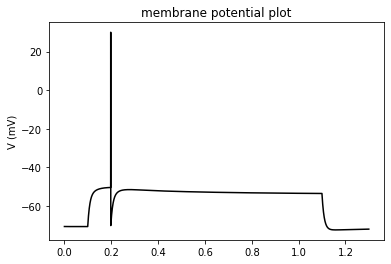
\includegraphics[width=0.25\linewidth]{figures/backend_check_files/backend_check_6_2.png}
%\caption{}

%\end{center}
%\end{figure}

%\begin{verbatim}
%    251 ms +- 5.02 ms per loop (mean +- std. dev. of 2 runs, 1 loop each)
%    240 ms +- 11.1 ms per loop (mean +- std. dev. of 2 runs, 1 loop each)
%    223 ms +- 12.5 ms per loop (mean +- std. dev. of 2 runs, 1 loop each)
%\end{verbatim}

\begin{verbatim}
    922 ms +- 12.7 ms per loop (mean +- std. dev. of 7 runs, 1 loop each)
\end{verbatim}

\subsection{Compare parallel to serial speeds, and accuracy}

Below is the Brian2/NeuralDynamics AdExp model. In-order to make the spike height greater than $0mV$ it was easier to use computer code to schedule waveform modifications that occur straight after the the brian2 simulation, these scheduled waveform modifications can be considered part of a peripheral shell of simulation code. In postprocessing
the waveform data type is a Neo Wave form object that is artificially the algorithm of determining rheobase and displaying results. The time of this model is determined on multiple factors, as discussed elsewhere, execution time is not uniform across model parameterizations. Models with multispiking behavior will take longer to solve.

Simulation times for this model vary, dramatically possibly because of
lazy evaluation, the simulation times may vary according to what else
you are running on your computer. Not all models experience a speed up when executed in parallel, however
this model was faster in the parallel Rheobase determination algorithm. Some common times are: $3.92,6.75,4.48,5.17$. Mean time was:

\subsection{Comparison of Times Taken to Find Rheobase}
Custom implementation JIT enabled implementation: $4.0s$. 
Brian2 taken to find Rheobase: $4.40s$ (serial), $3.976s$ (parallel).

The evaluation times between Brian2 and the custom written
integrator are similar. Both have average rheobase solution times of approximately 4 seconds, however the spike shape derived from the custom written integrator look more realistic under default paramaterizations. The biological plausibility of default model paramaterization has consequences for model optimization speed, because when  models undergo mutation and cross-over the mean of random models regressors towards the default model initialization, and if the default model is a bad fit to data, the average model sampled by the genetic algorithm will also be bad to data.\\

\begin{figure}
\begin{center}
\centering
  \centering
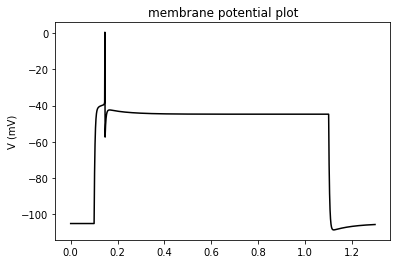
\includegraphics[scale=0.45]{figures/backend_check_files/backend_check_12_10}
\caption{Model parameterization of the brian2 simulator with the customization: interpolated spike height, forced to be above $0mV$}

  \label{fig:sub1}
  \centering
  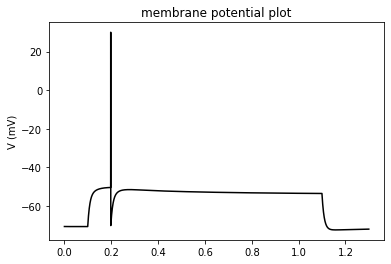
\includegraphics[scale=0.45]{figures/backend_check_files/backend_check_4_2}
    \caption{Default model parameterization of the custom written integrator}
  \label{fig:sub2}
\caption{Comparison between two Adxaptive Exponential Implementations}
\label{fig:test}
\end{center}
\end{figure}




    
$272 ms +- 66.5 $/mu$s per loop (mean +- std. dev. of 2 runs, 1$ loop each)

The next model to be evaluated is the NEURON Izhikevich model. The NEURON Izhikevich model has various draw backs. 1. It depends on an external file which must be recompiled each time this project is recreated. 2. The build environment of NEURON is non-trivial, and only a super dedicated NEURON modeller would install it on their system. Any performance advantage of using NEURON investment does not exceed the installation cost of installing the program. 3. The model implementation code is less generalizable than than the published Izhikevich model itself. Where the standard NEURON-NeuroML code only covers the Regular-Spiking model * This is likely due to a name space conflict between Capacitance. Neuron has a `capacitive' mechanism inside modelled Neurons, this particular model has section capacitance as well as an introduced capacitive term inside a C-compiled mechanism. Both contribute to a the membrane
potential calculation. * The NEURON Izhi model took $78$ seconds to find the rheobase current injection value $ 51.79367065 * pA $.

    
%\begin{center}
 %   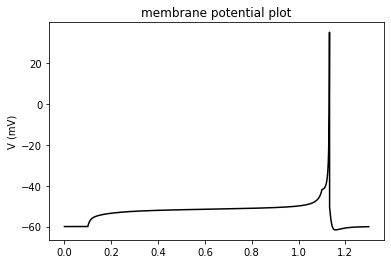
\includegraphics[width=0.7\textwidth,]{chapters/figures/backend_check_files/backend_check_14_2.png}
%    \caption{where is picture}
%\end{center}


%\begin{figure}
%    \centering
%    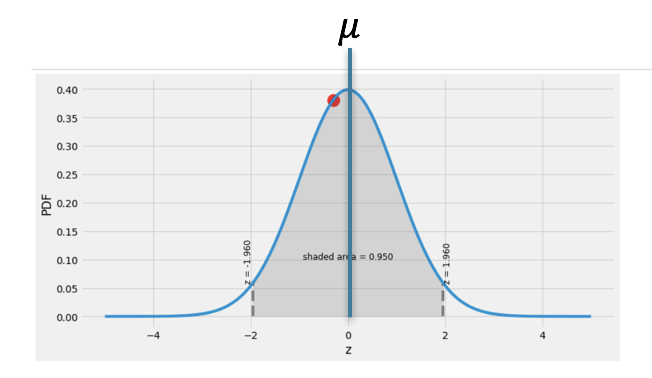
\includegraphics{chapters/normal_distribution}
%    \caption{This is your image%}
%    \label{fig:my_label}
%\end{figure}
%A tool numba JIT

% https://www.overleaf.com/learn/how-to/Images_not_showing_up 

        
The enabled forward Euler python Izhikevich model was very fast. The forward euler
implementation utilized Numba JIT \cite{lam2015numba}. Rheobase is found in under a second,
and in many cases close 0.5 seconds. This represents a very dramatic
speed up. Unlike the NEURON NeuroML implementation of the izhikitich equation,
this implementation is just as generalizable as the original MATLAB
implementation of the Izhikevich model, because it was possible to unify the fractured implementations in the one python simulator backend.


%\begin{verbatim}
%  time taken on
%  block 0.6859951019287109 \textbackslash{}n3.3 ms +- 9.79 %$\mu$s per loop (mean +- std. dev. of 2
%  runs, 100 loops each)\textbackslash{}n3.32 ms +- 30.9 us per loop (mean +- std. dev. of 2 runs,
%  100 loops each)\textbackslash{}n3.19 ms +- 10.9 us per loop (mean +- std. dev. of 2 runs, 100
%\end{verbatim}
        
\section{Python/LEMS and NEURON versions of single compartment Conducance Model.}

Conductance based models took approximately the same amount of
time to evaluate the Rheobase search algorithm as the python
implementation.

%This problem in the default parameterization of the python model was later located in the scale or units of capacitance, if default capacitance parameterization is multiplied by 100.0 the problem goes away.

time taken to compute rheobase $ 12.6s $

%\begin{center}
%\includegraphics{figures/backend_check_files/backen%d_check_22_2}
%\end{center}

%$ 1.40762329 * pA $


\subsection{NEURON versions of single compartment Conducance
model.}

%Hodgkin Huxley Conductance based channels models took approximately the same amount of time to evaluate the Rheobase search algorithm as the python implementation.

%The NEURON implementation was slightly faster, and the default parameterization of the model lacked `ringing'', or below threshold oscillations that the Python ODE version had under default conditions.

%This problem in the default parameterization of the python model was later located in the scale or units of capacitance, if default capacitance parameterization is multiplied by 100.0 the problem goes away.

Took $8.57$ seconds to find Rheobase.

The author also engineered GLIF model support for $NeuronUnit$ tests. In practice these models where hard to configure without expert knowledge, GLIF models contain the most parameters of all models, and many of these parameters are multi dimensional. GLIF models do not by necessity spike, interpolated spike times, are added in however, it does not make sense to evaluate GLIF models on spike shape features.

%which makes debugging their behavior very difficult. %None the less GLIF models where among the fastest to evaluate, and the author had success in making fitting these models to Allen Rheobase data.

    %\graphicspath{ {../figures/} }
%    \begin{center}
%    \begin{figure}
%    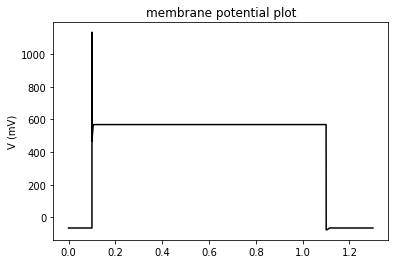
\includegraphics{figures/backend_check_files/backend_check_26_2}
    %kend_check_files/backend_check_26_2.png}
%    \end{figure}
    
%    \end{center}
%\begin{verbatim}
% 112.5 pA
%'value': array(1.40645904) * pA
%\end{verbatim}

% parameters of an adaptive exponential model
%\begin{verbatim}
%\{'El\_reference': -0.07016548013687134, %'C': 3.990452661875942e-10%,
%'init\_threshold': 0.02964956889477108, %'th\_inf': 0.02964956889477108,
%'spike\_cut\_length': 109.5, %'init\_voltage': -35.0, 'R\_input': %910258965.9792937\}
%\end{verbatim}
$ Rheobase = 112.5pA $

time taken to execute this model.
$ 0.23476457595825195 $

    


%$ 112.5 pA $
%$0.0 mV$ $-0.065 mV$

%    \begin{verbatim}
%    \{'value': array(183.33333333) * pA\}
%    \end{verbatim}

%\begin{verbatim}
%array(112.5) * pA
%\end{verbatim}


%\begin{verbatim}
%    0.017240506310425608 mV -0.08583939747094235 mV
%    0.017240506310425608 mV% -0.08583939747094235 mV
%\end{verbatim}

    %\begin{center}
    %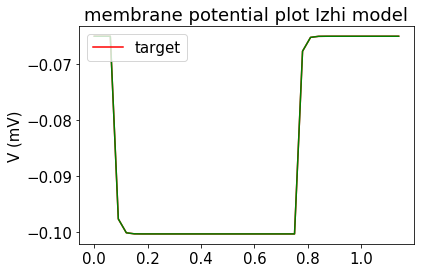
\includegraphics{figures/backend_check%_files/backend_check_32_2.png}
    %\end{center}
